%===================================== CHAP 1 =================================
\chapter{Introduction}

This chapter will introduce the thesis by providing a background for the problem and research area. It will also explain the motivation behind the thesis, and what we aspire to contribute to the field, before composing the problem into a set of research questions and objectives. The research methodology will be explained in terms of the research strategy, data generation methods and data analysis. Finally, the chapter will describe the structure of the thesis.

\section{Background}

\noindent The thesis is concerned with artificial neural networks (ANNs) and the use of visualization techniques to gain an understanding of their behaviour. Furthermore, the thesis explores a novel approach to improve the accuracy of facial recognition networks. The work presented in the thesis is a continuation from the results of the Specialization Project. \\

\noindent The expected outcome of the thesis can be divided into two parts:
\begin{enumerate}
    \item A visualization tool for deep learning
    \item A case study in facial recognition
\end{enumerate}

\noindent The first part proposes a tool for visualizing data produced during the training of an ANN. This visualization tool should be implemented in the form of a web interface where users can upload and run their Python scripts for creating and training such networks. The tool should use established visualization techniques to generate visualizations for the user in order to help them gain insight into why their networks behave as they do and, by extension, how they can be improved. A prototype of this interface has been implemented as part of the Specialization Project and will serve as a foundation for the continuation of the development. A description of the prototype, as well as an overview of the implementation details for the thesis, will be presented in chapter \ref{chap:implementation-chap}. \\

\noindent The case study in the second part explores whether it is possible to exploit facial expression data in order to improve an ANN for face recognition. The idea is that a network with access to facial expression data could learn the alterations of features associated with various expressions, and apply this to recognize faces which differ in the corresponding features. To examine the idea, a well known ANN architecture should be adapted to the face recognition domain to create two different networks: one conventional to act as a basis to be evaluated against and one experimental that exploits facial expression data.\\

\section{Motivation}

\noindent In the modern computer science landscape, ANNs are on the rise. They have enjoyed considerable success in a plethora of fields and there exist a multitude of frameworks dedicated to creating and training such networks. Among the frameworks are TensorFlow \cite{tensorflow2015-whitepaper} and Caffe2 \cite{caffe2}, which are open-source projects backed by tech giants Google and Facebook, respectively. However, an issue with ANNs is that they have been notoriously difficult to understand. Being dissatisfied with this knowledge vacuum, researchers have developed a number of visualization techniques to help gain insight into the inner workings of a network. Unfortunately, unlike the building of networks, there does not exist an extensive amount of options when it comes to facilitating the creation of visualizations. To combat this shortage, we aim to design and develop a tool that provides researchers with easy access to visualization techniques through a convenient user interface. More specifically, we plan to fill the void of an advanced visualization tool for the machine learning frameworks Theano \cite{theano} and TensorFlow through the use of Keras \cite{chollet2015keras}, a high-level API supporting both frameworks. The tool would aid researchers using these popular frameworks to gain a better understanding of their networks and how to improve them, thus enabling further research. \\

\noindent One of the fields where ANNs have been successfully applied is the area of face recognition. While notable performance has been achieved, research in the area of face recognition is not complete. Achieving robust facial recognition could provide an effective, non-intrusive biometric identification scheme that could be used for both information and physical security. Such identification systems would allow users to identify themselves with ease, without the use of passwords, PINs or ID cards, and gives organizations a hard-to-forge, human-independent security measure. Examples include computer logins, ATM access, airport security, and building access \cite{application_1, application_2, application_3}. We will therefore carry out a case study in the face recognition field, in addition to developing the visualization tool. We postulate that an approach that utilizes the information available in facial expressions may experience greater accuracy than one that tries to overcome expressions through invariance. \\


\section{Contributions}

The thesis introduces a visualization tool, implemented as a web interface, that can help researchers gain a better understanding of the behaviour of their ANNs and how to improve them. The effort will be concentrated on generating visualizations for networks whose input data reside in the image domain. The tool should be easily extensible, in regard to adding new visualization techniques and customizing the tool to a different machine learning framework. \\

\noindent The thesis also explores the face recognition field by investigating if the exploitation of facial expression data in face recognition systems could be beneficial. The results of the case study will indicate whether the approach has initial merit and should be researched further.

\section{Research Questions and Objectives} \label{sec:research-questions}

This section composes the problem stated into two research questions that will guide the problem solving process. We have also defined a set of research objectives that identifies the goals associated with each of the research questions. These goals must be achieved in order to be able to answer the questions.

\subsection{Visualization Tool}

We intend to aid researchers in the process of creating and training their ANNs. The research question is formulated as follows:

\begin{enumerate}[align=left, labelwidth=3.5em, leftmargin=!, itemindent=0em]
    \item[\textbf{RQ 1:}]How can we develop a visualization tool to improve the understanding of the behaviour of an artificial neural network?
\end{enumerate}

\noindent To answer this question, we will need to complete the following research objectives:

\begin{enumerate}[align=left, labelwidth=3.5em, leftmargin=!, itemindent=0em]
    \item[\textbf{RO 1.1:}] Examine existing tools in order to uncover shortcomings.
    \item[\textbf{RO 1.2:}] Identify visualization techniques that can be used to improve the understanding of an artificial neural network.
    \item[\textbf{RO 1.3:}]Develop a tool that incorporates the techniques found in 1.2 and addresses the shortcomings identified in 1.1.
\end{enumerate}

\subsection{Case Study in Face Recognition}

We aim to explore whether it is possible to exploit facial expression data in order to improve an ANN for face recognition. The research question is formulated as follows:

\begin{enumerate}[align=left, labelwidth=3.5em, leftmargin=!, itemindent=0em]
    \item[\textbf{RQ 2:}]How can facial expression data be utilized to improve a face recognition system?
\end{enumerate}

\noindent To answer this question, we will need to complete the following research objective:

\begin{enumerate}[align=left, labelwidth=3.5em, leftmargin=!, itemindent=0em]
    \item[\textbf{RO 2.1:}]Investigate how performance is affected when incorporating expression data in a face recognition system.
\end{enumerate}

\section{Research Methodology}

This section will explain the research method used in our thesis. Note that this is not to be confused with the more specific system development method, which is the explanation and documentation of how the suggested systems are implemented. The system development method will be addressed in chapter \ref{chap:implementation}. The research methodology is the combination of research strategies and data generation methods to be used in the thesis. Even though our research consists of two separate problems, we plan to address them simultaneously, and will employ similar methods for both. Thus, parts of this section discuss the research in general instead of separately for each research question.

\subsection{Research Strategy}

Oates \cite{oates} proposed six different strategies for answering research questions. Since both of our questions are concerned with the implementation of some kind of computer system, it is natural to employ the design and creation strategy, which focuses on developing new information technology (IT) products, or so called artefacts. March \& Smith \cite{march-smith} defines four types of IT artefacts: constructs, models, methods and instantiations. Instantiations are working systems demonstrating that constructs, models, methods, ideas or theories can be implemented in a computer-based system. The research output in our case will be two instantiations: the implemented visualization tool, and an implementation of a face recognition system incorporating a novel idea. \\

\noindent Vaishnavi \& Kuechler \cite{designscience} present an iterative process typical for design and creation, illustrated in \textbf{Fig. \ref{fig:dsr-cycle}}. The process suggests a "learning through making" approach and involves five steps, followed in an iterative cycle: awareness of problem, suggestion, development, evaluation and conclusion. The first step is to study existing literature and research to uncover the need for something. The second step provides a creative leap from the need to a simple idea of a solution. Then, the idea is implemented in the third step, followed by an evaluation of this implementation and an explanation of possible deviations from the expectation in the fourth step. Finally, in the fifth step, the result is documented, and the knowledge gained, as well as any possible future work, is identified. \\

\begin{figure}[h!]
    \centering
        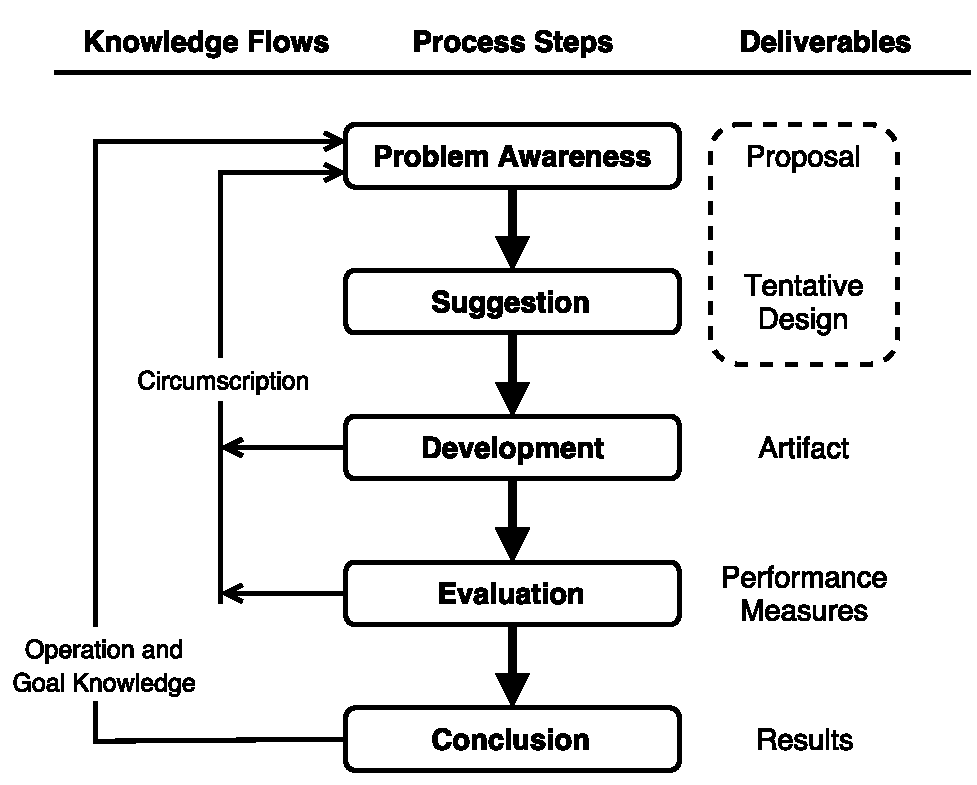
\includegraphics[width=0.7\textwidth]{fig/dsr-cycle.pdf}
        \caption{Research Process Model}
        \label{fig:dsr-cycle}
\end{figure}

\noindent For the visualization tool, the first couple of iterations of this cycle have already been conducted in the Specialization Project. The result of this project included many pointers to future work, which will be addressed in this thesis. We will continue to repeat the process until we can conclude with an implementation that is satisfactory according to our research question and objectives. For the case study, however, no development was conducted in the Specialization Project. The focus was rather on the first two steps, namely to define the problem and suggest a solution. In this thesis, we will continue the process by implementing a suggested solution, and continue to evaluate and improve it until we reach a conclusion.\\

\subsection{Data Generation Methods} \label{sec:data-generation-methods}

The data that will be used in the thesis will mainly be qualitative data in the form of documents. For the implementation of the visualization tool, articles on various visualization techniques that can aid in understanding ANNs will be essential. We will also make use of documentation of the frameworks and technologies used in implementation. To document the implemented tool and capture our research strategy, we will generate our own documents using architectural diagrams and user manuals. \\

\noindent For the case study, we will need a large amount of images. Since our case study is concerned with the field of face recognition with expressions, we require images of people with different facial expressions, photographed under various conditions, that are labeled with identification and expression. There exist several datasets created solely for the purpose of face recognition, but the challenge will be to find one of appropriate size, containing the required labels. Unfortunately, the larger datasets examined have a tendency to be expensive or lack availability. The chosen dataset will be used to both train the networks and validate their performance afterwards.

\subsection{Data Analysis}

To present the results of the visualization tool, we will make use of well known ANNs, and show the visualizations produced at various stages of training. Since the results are images, we will need to perform quantitative data analysis on these images. The goal will be to identify connections between the visualizations and the behaviour of the networks, both in terms of why they may perform well and why they may struggle. \\

\noindent Qualitative data analysis will be performed on the results of the case study. The prediction accuracy of an ANN is defined as the percent of correctly classified inputs, in our case images. The accuracy of our implemented network incorporating the proposed modification will be measured against the accuracy of the baseline network. By comparing these, we should be able to determine whether exploiting expressions in such a way could be beneficial.

\section{Thesis Structure}

\textbf{Table \ref{tab:thesis-structure}} presents an overview of the structure of the thesis.

\begin{table}[!h]
\begin{center}
\begin{tabular}{ | l | p{8cm} |}
\hline
\textbf{Chapter/Appendix} & \textbf{Description} \\ \hline
1. Introduction & An overview of the research to be done in the thesis. \\ \hline
2. Background Theory & The theory relevant for the thesis. \\ \hline
3. Related Work & An overview of related work. \\ \hline
4. Implementation & The implementation of the visualization tool and case study in terms of methods and architecture. \\ \hline
5. Results & The results from both the visualizations and the case study. \\ \hline
6. Discussion & Discussion of the results presented in the previous chapter. \\ \hline
7. Conclusion and Future Work & A short conclusion and some pointers to future work. \\ \hline
A. Installation \& Setup & A step by step wizard on how to install and set up the visualization tool. \\ \hline
B. User Manual & How to use the visualization tool, including screenshots of the GUI. \\ \hline
C. Callbacks API & An API for the callbacks to be used with the visualization tool. \\ \hline
D. Visualization Files & A note on the format of the content of the visualization files. \\ \hline
\end{tabular}
\end{center}
\caption{Overview of the thesis structure}
\label{tab:thesis-structure}
\end{table}

\cleardoublepage